\IEEEraisesectionheading{\section{Introduction}\label{sec:introduction}}

Deep Convolutional Neural Networks (DCNNs) \cite{LeCun1998} have 
pushed the performance of computer vision systems to soaring heights on a
broad array of high-level problems, including image classification
\cite{KrizhevskyNIPS2013, sermanet2013overfeat, simonyan2014very,
  szegedy2014going, papandreou2014untangling} and object detection
\cite{girshick2014rcnn, erhan2014scalable, girshick2015fast, ren2015faster,
  he2015deep, liu2015ssd}, where DCNNs trained
in an end-to-end manner have delivered strikingly better results than systems relying
on hand-crafted features.
%
Essential to this success is the built-in invariance of DCNNs
to local image transformations, which allows them to learn increasingly
 abstract data representations \cite{zeiler2014visualizing}. This
invariance is clearly desirable for classification tasks, but can hamper
dense prediction tasks such as semantic segmentation, where abstraction of spatial
information is undesired.

In particular we consider three challenges in the application of DCNNs to semantic image segmentation: (1) reduced feature resolution,
(2) existence of objects at multiple scales, and (3) reduced localization
accuracy due to DCNN invariance. Next, we discuss these challenges and our
approach to overcome them in our proposed DeepLab system.

The first challenge is caused by the repeated combination of max-pooling and downsampling (`striding')
 performed at consecutive layers of  DCNNs originally designed
for image classification \cite{KrizhevskyNIPS2013, simonyan2014very, szegedy2014going}.
This results in feature maps with significantly reduced spatial resolution when
the DCNN is employed in a fully convolutional fashion \cite{long2014fully}. In
order to overcome this hurdle and efficiently produce denser feature maps, we
remove the downsampling operator from the last few max pooling layers of DCNNs
and instead {\it upsample the filters} in subsequent convolutional layers, resulting
in feature maps computed at a higher sampling rate. Filter upsampling amounts to
inserting holes (`trous' in French) between nonzero filter taps. This technique has a long history in signal processing,
originally developed for the efficient computation of the undecimated wavelet
transform in a scheme also known as ``algorithme \`a trous''
\cite{holschneider1989real}. We use the term \emph{atrous convolution} as a shorthand for convolution with
upsampled filters. 
Various flavors of this idea have been used before
in the context of DCNNs by \cite{giusti2013fast, sermanet2013overfeat,
papandreou2014untangling}. In practice, we recover full resolution feature maps
by a combination of atrous convolution, which computes feature maps more
densely, followed by simple bilinear interpolation of the feature responses to
the original image size. This scheme offers a simple yet powerful alternative to
using deconvolutional layers \cite{zeiler2014visualizing, long2014fully} in
dense prediction tasks. Compared to regular convolution with larger filters, atrous
convolution allows us to effectively enlarge the field of view of filters without
increasing the number of parameters or the amount of computation.

The second challenge is caused by the existence of objects at
multiple scales. A standard way to deal with this is to present to the DCNN
rescaled versions of the same image and then aggregate the feature or score maps
\cite{papandreou2014untangling, chen2015attention,kokkinos2016pushing}. We show that this approach
indeed increases the performance of our system, but comes at the cost of computing feature
responses at all DCNN layers for multiple scaled versions of the input image. Instead, motivated
by  spatial pyramid pooling \cite{lazebnik2006beyond, he2014spatial},
we propose a computationally efficient scheme of resampling a given feature layer at multiple
rates prior to  convolution. This amounts to probing the original image with multiple filters
that have complementary effective fields of view, thus capturing objects as
well as useful image context at multiple scales. Rather than actually resampling features, 
we efficiently implement this mapping using
multiple parallel atrous convolutional layers with different sampling
rates; we call the proposed technique ``atrous spatial pyramid pooling'' (ASPP).

The third challenge relates to the fact that an object-centric classifier 
requires invariance to spatial transformations, inherently
limiting the spatial accuracy of a DCNN. One way to mitigate this
problem is to use skip-layers to extract ``hyper-column'' features from multiple network layers when
computing the final segmentation result
\cite{hariharan2014hypercolumns, long2014fully}. Our work explores an
alternative approach which we show to be highly effective. In particular, we
boost our model's ability to capture fine details by employing a fully-connected
Conditional Random Field (CRF) \cite{krahenbuhl2011efficient}. CRFs have been
broadly used in semantic segmentation to combine class scores computed by
multi-way classifiers with the low-level information captured by the local
interactions of pixels and edges
\cite{rother2004grabcut, shotton2009textonboost} or superpixels
\cite{lucchi2011spatial}. Even though works of increased sophistication have
been proposed to model the hierarchical dependency \cite{he2004multiscale,
  ladicky2009associative, lempitsky2011pylon} and/or high-order dependencies
of segments \cite{delong2012fast, gonfaus2010harmony, kohli2009robust, CPY13, Wang15}, we
use the fully connected pairwise CRF proposed by
\cite{krahenbuhl2011efficient} for its efficient computation, and ability to
capture fine edge details while also catering for long range dependencies. That
model was shown in \cite{krahenbuhl2011efficient} to improve the performance of
a boosting-based pixel-level classifier. In this work, we demonstrate that it
leads to state-of-the-art results when coupled with a DCNN-based pixel-level
classifier.

\begin{figure*}[!th]
  \centering
  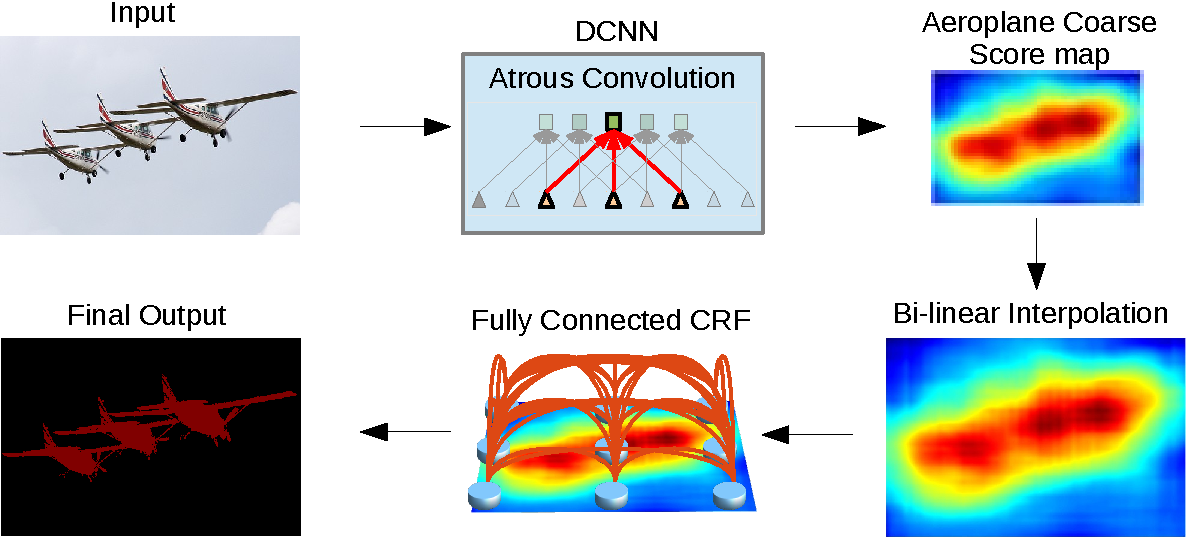
\includegraphics[width=0.7\linewidth]{fig/model_illustration4.pdf}
  \caption{Model Illustration. A Deep Convolutional Neural Network such as
  VGG-16 or ResNet-101 is employed in a fully convolutional fashion, using
  atrous convolution to reduce the degree of signal downsampling (from 32x
  down 8x). A bilinear interpolation stage enlarges the feature maps to the
  original image resolution. A fully connected CRF is then applied to refine
  the segmentation result and better capture the object boundaries.}
  \label{fig:ModelIllustration}
\end{figure*}

A high-level illustration of the proposed DeepLab model is shown in
\figref{fig:ModelIllustration}. A deep convolutional neural network
(VGG-16 \cite{simonyan2014very} or ResNet-101 \cite{he2015deep} in this work)
trained in the task of image classification is re-purposed to the task of
semantic segmentation by (1) transforming all the fully connected layers
to convolutional layers (\ie, fully convolutional network \cite{long2014fully})
and (2) increasing feature resolution through
atrous convolutional layers, allowing us  to compute feature
responses  every 8 pixels instead of every 32 pixels in the original network. 
We then employ bi-linear interpolation to upsample by a
factor of 8 the score map to reach the original image resolution, yielding the 
input to 
a fully-connected CRF \cite{krahenbuhl2011efficient} that refines the
segmentation results.

From a practical standpoint, the three main advantages of our DeepLab
system are: (1) Speed: by virtue of atrous convolution, our dense DCNN operates
at 8 FPS on an NVidia Titan X GPU, while Mean Field Inference for the
fully-connected CRF requires 0.5 secs on a CPU. (2) Accuracy: we obtain
state-of-art results on several challenging datasets, including the PASCAL VOC 2012
semantic segmentation benchmark \cite{everingham2014pascal}, PASCAL-Context
\cite{mottaghi2014role}, PASCAL-Person-Part \cite{chen_cvpr14}, and Cityscapes
\cite{Cordts2016Cityscapes}. (3) Simplicity: our system is composed of a cascade of
two very well-established modules, DCNNs and CRFs.
% and is trained end-to-end with one pass.
%, instead of several steps as other state-of-art models.

The updated DeepLab system we present in this paper features several
improvements compared to its first version reported in our original conference
publication \cite{chen2014semantic}. Our new version can better segment objects
at multiple scales, via either multi-scale input processing \cite{farabet2013learning, lin2015efficient, chen2015attention} or the 
proposed ASPP. We have built a residual net variant of DeepLab by adapting
the state-of-art ResNet \cite{he2015deep} image classification DCNN, achieving
better semantic segmentation performance compared to our original model based on
VGG-16 \cite{simonyan2014very}. Finally, we present a more comprehensive
experimental evaluation of multiple model variants and report state-of-art
results not only on the PASCAL VOC 2012 benchmark but also on other challenging
tasks. We have implemented the proposed methods by extending
the Caffe framework \cite{jia2014caffe}. We share our code and models at a
companion web site \url{http://liangchiehchen.com/projects/DeepLab.html}.


%We have publicly released the complete source code for this project and
%many other groups have used or extended our earlier system.  
%We will share the updated version of our system presented here in a forthcoming
%code release.

%In particular, when compared to a broad pool of works recently developed around the problem of combining DCNNs with semantic segmentation, our system can be understood as being substantially simpler, relying on a minimal number of components, while at the same time delivering state-of-the-art results.
%\cite{mostajabi2014feedforward} 
